\documentclass{cmspaper}
\def\RCS$#1: #2 ${\expandafter\def\csname RCS#1\endcsname{#2}}
\RCS$Revision: 1.14 $
\RCS$Date: 2005/09/03 22:28:58 $

\usepackage{graphicx}

\begin{document}
\begin{titlepage}
  \whitepaper
  \date{Revision \RCSRevision, \RCSDate}
  \title{PhEDEx TMDB Schema and Database Interactions}

  \begin{Authlist}
    Tim~Barrass, Simon~Metson\Instfoot{bristol}{University of Bristol, Bristol, UK}
    Lassi~A.~Tuura\Instfoot{neu}{Northeastern University, Boston, USA}
  \end{Authlist}

  \begin{abstract}
    This white paper describes the database schema used by PhEDEx,
    the data placement and transfer system used by CMS.  It also
    defines the expected set of agent-TMDB interactions, effectively
    outlining the functionality of the main agents.
  \end{abstract}

  \note{Schema version V2.2}
\end{titlepage}

\setcounter{page}{2}

%%%%%%%%%%%%%%%%%%%%%%%%%%%%%%%%%%%%%%%%%%%%%%%%%%%%%%%%%%%%%%%%%%%%%%
\section{Transfer Management Database}

%FIXME: Update picture!
%\begin{figure}[htbp]
%\centering
%  \includegraphics[width=15cm]{tmdb-schema.eps}
%  \caption{Entities and relations in the TMDB V2.  The SQL to
%   create the schema is available in the "Schema" subdirectory.}
%   \label{fig:schema}
%\end{figure}

\begin{description}
  \item [\texttt{t\_node}]\mbox{}

    A reference against which node names are constrained to exist
    and to be unique.

  \item [\texttt{t\_node\_import}]\mbox{}
  
    The protocols with which the node can import files, ordered by
    preference.  In general \texttt{gsiftp} is required to be listed
    as the lowest common denominator.
  
  \item [\texttt{t\_node\_export}]\mbox{}
  
    The protocols with which the node can export files.  In general
    \texttt{gsiftp} is required to be listed as the lowest common
    denominator.

  \item [\texttt{t\_node\_neighbour}]\mbox{}

    The neighbour relationships of the nodes.  This information is
    static and modified by the transfer system administrators.

  \item [\texttt{t\_routing}]\mbox{}

    Node routing tables.  In theory each node's routing tables are
    private to that node, we simply smash all the data into one table.
    The routing algorithm is described in a separate white paper.
    This information is dynamic: it is produced by the routing agents
    based on \texttt{t\_node\_neighbour} at run time.

  \item [\texttt{t\_agent}]\mbox{}

    Provides a reference against which agent names can be checked.

  \item [\texttt{t\_agent\_status}]\mbox{}

    Indication of last contact by an agent at a particular site.
    Used to monitor the availability of the agents and/or sites.

  \item [\texttt{t\_agent\_messages}]\mbox{}

    Simple steering messages to agents: {\em resume}, {\em suspend},
    {\em stop} and {\em go away}.  These can be used for scheduled
    interventions, a global manager might post {\em T1 : SUSPEND :
    A : Download } to suspend downloads at node A at the time T1.
    The agent, or an automatic manager of it, would suspend.
    Handled messages that are not permanent are removed.

  \item [\texttt{t\_file}]\mbox{}

    An entry for a file available for distribution.  This records
    some core attributes about each file: GUID, LFN, file size,
    checksum, when and where the file was first injected, the
    main logical groupings the file belongs into, and so on.  An
    entry matching the file's logical grouping, called {\em block},
    is required in \texttt{t\_block}.

  \item [\texttt{t\_file\_attributes}]\mbox{}

    Additional meta data attributes about each file, recorded as
    (attribute, value) pairs per GUID.  This holds extra information
    about the file which PhEDEx carries for clients but does not use
    itself.  The table format allows attributes to be added and
    removed without modifying the schema.  CMS uses it to store the
    POOL meta data attributes for a file.

  \item [\texttt{t\_replica\_state}]\mbox{}
  
    A replica of a file at a location.  An entry in this table
    represents the fact that a copy of the file exists at this
    location.  A file appears in this table as many times as
    there are replicas of it.  Note that collapsed blocks will
    cause this table to have less rows than there are files at
    the node.

  \item [\texttt{t\_transfer\_state}]\mbox{}

    A transfer assignment of a file.  An entry in this table represents
    the progress of making another replica of file, from a specific
    source replica (\texttt{from\_node}) to a specific destination
    replica (\texttt{to\_node}).  A completed transfer leads to the
    destination replica getting created in \texttt{t\_replica\_state}.

    During the transfer a file goes through a certain set of states.
    There are separate states for the file at source and destination,
    and the ``download handshake'' specifies the progression through
    the two.  The available source states are {\em unavailable} (0)
    and {\em available} (1).  The possible destination states are
    {\em assigned} (0), {\em wanted} (1), {\em in transfer} (2),
    {\em transferred} (3), {\em error} (100+) or {\em agent- or
     site-specific} (4-100).  Only certain progressions of source
    and destination states are allowed as explained below.
    
    Completed transfers are removed and archived into the next
    table, \texttt{t\_transfer\_completed}

  \item [\texttt{t\_transfer\_completed}]\mbox{}

    Completed transfers.  This is filled automatically from either
    transfers or by a cleaning agent.  This is only a temporary
    storage area; the results are eventually aggregated into the
    performance table \texttt{t\_perf\_histogram} and then deleted.

  \item [\texttt{t\_transfer\_tracking}]\mbox{}

    Temporary detail information about the state progression of each
    file in \texttt{t\_transfer\_state}.  A database trigger inserts
    a row in the tracking table for each insertion and update of the
    transfer state table.  Source for \texttt{t\_quality\_histogram}
    updates, then copied to \texttt{t\_transfer\_history}.

  \item [\texttt{t\_transfer\_history}]\mbox{}

    Detailed historical information about the state progression of
    each file in \texttt{t\_transfer\_state}.  The table is updated
    from \texttt{t\_transfer\_tracking}; old entries are archived
    monthly.

  \item [\texttt{t\_perf\_histogram}]\mbox{}

    Aggregated transfer performance information.  This table records
    for each 5-minute period the amount of transfers completed and
    the still pending, for each pair of nodes where transfers are
    either scheduled or taking place.  The table records aggregate
    information -- the number of files and the total size -- not
    the actual identity of the files.  The information is updated
    automatically from the contents of the other tables
    (\texttt{t\_transfer\_state}, \texttt{t\_transfer\_completed}).
    Apart from the agent logs and the transfer history table, this
    is the only long-term memory kept about the transfers in the
    database.

  \item [\texttt{t\_quality\_histogram}]\mbox{}

    Aggregated transfer quality information.  This table records
    for each 5-minute period and pair of nodes the count of file
    transfer state transitions which had to do with either file
    transfer start or end.  The information is aggregated; the
    starts and ends are only counted, not correlated.  The table
    is filled by processing \texttt{t\_transfer\_tracking}, after
    which the rows are copied into \texttt{t\_transfer\_history}.

  \item [\texttt{t\_subscription}]\mbox{}

    Data subscriptions.

  \item [\texttt{t\_block}]\mbox{}

    Identifies logical file groupings called blocks.  A block of
    files can be ``open'' or ``closed''; an open block can have
    files added to it, a closed block is frozen and cannot be
    changed.  Open blocks cannot be collapsed (see below), while
    closed ones can be.

  \item [\texttt{t\_block\_replica}]\mbox{}

    Similar to \texttt{t\_replica\_state}, but for entire blocks of
    files.  Tracks how many files in the block have been destined
    to the node, are at the node, or are in transfer to or from
    the node.  When all replicas of the block have suitable state
    (no partial blocks, no files in transfer, subscribed files at
    the destination), the block is ``deactivated:'' the replica
    entries are removed from \texttt{t\_replica\_state}.

  \item [\texttt{t\_block\_destination}]\mbox{}

    Transfer destination assigned for a block of file.  A block
    appears in this table for each destination the files in it
    should be transferred to.  Note that these are {\em final}
    destinations, intermediate nodes on the way to the
    destination are not recorded here.  Has a time stamp to
    indicate when the block has reached the destination in its
    entirety.

  \item [\texttt{t\_authorisation}]\mbox{}

    Record of site contacts and which database access roles they
    have been granted.  This is used in administering the system,
    not by the agents.
    
  \item [\texttt{t\_info\_agent\_status}]\mbox{}

    Information about the agents running at each site.  Exposes
    limited information about the agents, such as the computer
    they run on, the path to the state directory, and unix process
    id, which facilitate debugging interactions with the database.
    For drop box agents also reports the number of drops in their
    various states.

  \item [Other \texttt{t\_info\_*}]\mbox{}

    Information gathered on the background from the other tables.
    Most of these tables record statistics for quick access from
    monitoring tools and web browsers.  The data is refreshed
    periodically by administrative agents.

  \item [\texttt{t\_transfer\_summary}]\mbox{}
  
    Information we hope to gather one day, or an alternative form
    for \texttt{t\_transfer\_state}.  Not used.

  \item [\texttt{t\_dsb\_*}]\mbox{}
  
    Test playground for a prototype dataset bookkeeping system,
    for caching information from CMS RefDB for more convenient
    use.  Not used by the transfer system at all, and could and
    should be moved into entirely separate database.

  \item [\texttt{t\_request\_*}]\mbox{}
  
    Test playground for managing higher-level data placement
    requests, ``transfer requests.''  Not used by the transfer
    system at all, and could and should be moved into entirely
    separate database.

\end{description}

%%%%%%%%%%%%%%%%%%%%%%%%%%%%%%%%%%%%%%%%%%%%%%%%%%%%%%%%%%%%%%%%%%%%%%
\section{Registration and removal of network components}

The registration and removal of network components, ``nodes,'' is dealt with in detail in a separate ``Routing'' white paper.

%%%%%%%%%%%%%%%%%%%%%%%%%%%%%%%%%%%%%%%%%%%%%%%%%%%%%%%%%%%%%%%%%%%%%%
\section{Agents}

%%%%%%%%%%
\subsection{Typical agent-transfer management database communication}

The following discussion is intended to give a feel for the flow of data through the system. The functionality of the agents can basically be defined in terms of these interactions.

%%%%%%%%%%
\subsection{Deploying generic agent SQL as PL/SQL}

[ If all agents use the same queries, are these very valid candidates for PL/SQL server side processes to increase performance?  Our agents use long-lasting database connections and maximise the use of place-holder variables to avoid database server hard parse, and mostly execute single SQL statements, so PL/SQL would not give great advantages.  However certain operations involve significant amount of procedural logic, e.g. file routing, and using server side code might be justified. ]

%%%%%%%%%%
\subsection{Publishing agent availability}

Every time an agent is available, it should publish that it is indeed operational.  ``Available'' means in this context that the agent is running and able to carry out its task, so an agent should not be updating its status if it is busy doing something else, such as in the middle of a large operation that will make it unable to respond to other requests.

{\small\begin{verbatim}
  insert into t_agent values (:agentname);

  insert into t_agent_status values
  (:now, :mynode, :agentname, 1);

  update t_agent_status set
    state = 1, timestamp = :now
  where node = :mynode and agent = :agentname;
\end{verbatim}}

\subsection{Checking for agent messages}

This is a  method for sending simple global configuration and coordination messages to the nodes.  The messages are simply ``restart,'' ``suspend,'' and ``stop'', plus ``go away'' for a permanent stop (see table \ref{table:messages}).

\begin{table}
\centering
\begin{tabular}[!h]{|c|c|l|} 
\hline Message  & Action to take
\\ \hline
	RESTART & Indication for agent operator to restart agents.
\\	SUSPEND & Agent should stay alive but do nothing.
\\	STOP    & Agent should stop and exit.
\\	GOAWAY  & Agent should stop and exit.
\\ \hline
\end{tabular}
\caption{Simple coordination messages passed to agents via \texttt{t\_agent\_message} table.}
\label{table:messages}
\end{table}

The agent should only consider messages that are in the past; future messages should not be processed.  This is to allow for scheduled interventions.

The processing of the messages is as follows.  A RESTART message overrides any previous SUSPEND, STOP or GOAWAY message, and indicates the agent can be restarted (in case of STOP or GOAWAY), or resumed (in case of SUSPEND).  Once a RESTART has been processed, all messages older than it can be removed.  The STOP message simply causes the agent to exit; it should remove the message before exiting.  The GOAWAY is similar to STOP, but is not removed, thus leaving it in the database and preventing agents from starting until the time of a RESTART.  The SUSPEND message should cause the agent go on hold, and periodically check for further messages.

{\small\begin{verbatim}
  select timestamp, message
  from t_agent_message
  where node = :mynode and agent = :me
  order by timestamp asc;
\end{verbatim}}

To delete message \texttt{msg} at time \texttt{t}, and anything that preceded it:

{\small\begin{verbatim}
  delete from t_agent_message
  where node = :node and agent = :me
  and (timestamp < :t or (timestamp = :t and message = :msg));
\end{verbatim}}


%%%%%%%%%%%%%%%%%%%%%%%%%%%%%%%%%%%%%%%%%%%%%%%%%%%%%%%%%%%%%%%%%%%%%%
\section{File states and the download handshake}

The possible source states (\texttt{t\_transfer\_state.from\_state}) for a file are: {\em unavailable} (0) and {\em available} (1).

The possible destination states (\texttt{t\_transfer\_state.to\_state}) for a file are: {\em assigned} (0), {\em wanted} (1), {\em in transfer} (2), {\em transferred} (3), {\em error} (100+) or {\em agent- or site-specific} (4-99).

Both source and destination states have time stamp attributes associated with them.  When the state value is changed, the time stamp must be updated to the UTC time of the update operation.

The transfer handshake proceeds as follows.  When a file router creates a transfer assignment, it initialises the row to the ``unavailable, assigned'' state (\texttt{from\_state} = \texttt{to\_state} = 0).  When the destination download agent wants to download the file, it must first mark it in \texttt{to\_state} = 1, ``wanted.''  It must refresh the wanted state at least once every 15 minutes to indicate continued interest in the file; wanted files older than this are ignored by the export side, on the assumption the agent is not capable of receiving files any more.

At any time the exporting side may mark an unavailable file in \texttt{from\_state} = 1, ``available,'' meaning that the file is readily accessible, such as staged on disk.  Before marking the file available the export side must provide a transfer name, \texttt{from\_pfn}.  If the file ceases to be readily accessible, it can be marked back into ``unavailable'' state, \texttt{from\_state} = 0, optionally also clearing out \texttt{from\_pfn}, but only if it is not already in transfer: \texttt{to\_state} must be 0 or 1.

When the file has been marked as available for transfer (\texttt{from\_state} = 1), and regardless of whether the download previously marked it as ``wanted,'' the agent may proceed to transfer the file.  The source PFN to use for the transfer is provided in \texttt{from\_pfn}.  When the transfer has been started, the file must be marked into \texttt{to\_state} = 2, ``in transfer.''  When the transfer is completed, the file is put into \texttt{to\_state} = 3, ``transferred,'' if the transfer was successful, or an error state, \texttt{to\_state} >= 100, if the transfer failed.  Files in error state must be brought back into \texttt{to\_state} = 0 or 1, assigned or wanted, before re-attempting download.  The canonical implementation is that the error state given also encodes the ``cool-off'' period assigned to the file before a download is attempted again, for example 109 for 9-minute cool-off period, 115 for 15-minute period and so on.

Destination states between 4 and 99 inclusive are available for custom agent behaviour, as long as the use of the states does not interfere with the above handshake.

Transferred files in \texttt{to\_state} = 3 are automatically archived by a maintenance agent into the \texttt{t\_transfer\_completed} table.  To reduce query load on \texttt{t\_transfer\_state} we recommend that each agent completing a transfer itself moves the row over.  In this case, the file must first be marked in \texttt{to\_state} = 3, then immediately inserted to the other table and removed from the transfer state table.  The update of \texttt{to\_state} is required in order to make sure that \texttt{t\_transfer\_history}, updated by a trigger on \texttt{t\_transfer\_state}, records correct information.

When selecting files to download, it is recommended to group by \texttt{t\_file.inblock} and \texttt{t\_file.insubblock}.  This will group files that ``belong together'' at destination, in particular significantly increasing the likelyhood that they will end up on the same tape.  Also when the receiving client desires to use the files before entire large blocks have been copied, ordering by the sub-block level ensures related files, typically required together, arrive all roughly at the same time -- if the client requires files in bundles of three, downloading one file from each bundle would be considerably worse for the client than grouping the files by those groups of three.

The order in which different \texttt{inblock} or \texttt{insubblock} values are selected is however {\em not} important.  In fact it is a good idea to randomise the relative order of \texttt{inblock} and \texttt{insubblock} instead of using a fixed, e.g. alphabetical, order.  This will cause downloads from different sites to ``spread,'' making it likely they each download a different set of files.  This allows the receivers then make those files available for other interested parties; when several sites want the same set of files from a single location, this allows the download charge to even out.  Such randomisation does not generally have adverse effect on the exporting side, as the exporter can see long-term download charge (that is, ``wanted'' files) and make educated stage-in requests.  In any case the download agents will download files in the order the exporting side makes them available, not in the order they asked for the files.

%%%%%%%%%%%%%%%%%%%%%%%%%%%%%%%%%%%%%%%%%%%%%%%%%%%%%%%%%%%%%%%%%%%%%%
\section{Data sources}

\subsection{Injecting files into transfer}

To make a file available for distribution, three steps must be carried out.  Firstly, the block into which the file belongs to must be created or updated, the file must be added together with metadata attribute information associated with it, and replicas must be created for the nodes where the file exists.

\subsection{Creating or updating a file block}

If no file block yet exists for the file, the injector must first create a block.

{\small\begin{verbatim}
  insert into t_block values
  (:timestamp, :name, :owner, :dataset,
   :files, :bytes, :isopen);
\end{verbatim}}

Here, \texttt{timestamp} is current time in UTC, \texttt{name} is the name of the file block (in CMS, "owner/dataset"), \texttt{owner} and \texttt{dataset} are the CMS data class properties, \texttt{files} is the number of files in the block, \texttt{bytes} the sum total of the file sizes in the block, and \texttt{isopen} is 1 if the block is open, or zero if it is closed.

If the files being added are truly new, then \texttt{files} and \texttt{bytes} would start out as one and the size of the file being injected, respectively, and \texttt{isopen} must be 1.

If the block is new, it is not necessary to lock it provided the transaction is not committed.  Once the transaction has been committed, the block must be locked before making any other changes.

\subsection{Locking and updating a block}

If the injector is adding a file to an already existing block, it must lock the block before making any other changes.  The locking is mandatory, and important to get right; it is the only way to guarantee that various block-level operations are working with correct state.  Note that once the block has been locked, all changes must be consistent by the time commit occurs.

{\small\begin{verbatim}
  select * from t_block
  where name = :name
  for update
\end{verbatim}}

Once the block has been locked, the injector must ensure that the block is not closed: \texttt{isopen} must be non-zero.  If the block is closed, the whole block, including all the block replicas, must be deactivated before new files can be added.  If the block is open, the injector can proceed to add the file(s).

Note that every time the transaction is committed, the lock is lost, and the injector must re-acquire the lock and perform all the checks mentioned above.

\subsection{Adding files}

To make files available for distribution, they are added together with their attributes:

{\small\begin{verbatim}
  update t_block set
    files = files + 1,
    bytes = bytes + :filesize
  where name = :inblock;

  insert into t_file values
    (:timestamp, :guid, :node, :inblock, :insubblock,
     :lfn, :filetype, :filesize, :checksum);

  insert into t_file_attributes values
    (:guid, :attr, :value);
\end{verbatim}}

Here, \texttt{timestamp} is the UTC time at the time of injection, \texttt{guid} the file's unique identifier, and the key by which PhEDEx identifies the file.  The \texttt{node} is the PhEDEx node where the injection is being done, and must refer to a name in \texttt{t\_node}.  The rest of the values are various properties of the file.  The \texttt{inblock} and \texttt{insubblock} are groupings of the file; the former refers to \texttt{t\_block.name}, but the latter is purely informational, though see the download handshake description for uses of it.  The \texttt{lfn} and \texttt{filetype} are the logical file name and some description of the type of the file that may be useful for clients, respectively; PhEDEx only transmits them through from source to destination without ever using them itself.  The \texttt{filesize} is the size of the file in bytes, and \texttt{checksum} the CRC-32 checksum of the file as computed by the unix \texttt{cksum} utility.  While PhEDEx does not use either itself, the file size is frequently used in post-transfer verification scripts, and the checksum sometimes.

The injector is required to make sure that \texttt{t\_block} and \texttt{t\_file} are consistent on the count of files in a block and the sum of their sizes.

The injector can also add any number of key, value pairs of information about the file into \texttt{t\_file\_attributes}.  The attributes are not used by PhEDEx at all, only passed to whoever wants access to them.  CMS uses them to store the POOL file catalogue information.


%%%%%%%%%%%%%%%%%%%%%%%%%%%%%%%%%%%%%%%%%%%%%%%%%%%%%%%%%%%%%%%%%%%%%%
\section{Data placement}

\subsection{Allocator agent and distribution management}

The allocator agent regularly scans \texttt{t\_block} and assigns each block to destinations using \texttt{t\_subscriptions}.  The destinations are determined using the ``data stream'' attributes (currently hardcoded as CMS' ``dataset'' and ``owner'', which ought to be fixed).  For each block and destination not already mentioned in \texttt{t\_block\_destination} the allocator agent creates a new ``open,'' that is not completed, allocation.

{\small\begin{verbatim}
  select b.name, s.destination
  from t_block b
  join t_subscription s
    on s.owner = b.owner and s.dataset = b.dataset;

  insert into t_block_destination values
  (:timestamp, :blockname, :destination_node, null)
\end{verbatim}}

In the past we have used allocator agent which redirected files to fallback destinations if the primary one was unable to receive files at sufficient rate.  In the V2.2 schema the same task could be done by by checking for \texttt{t\_block\_destination} allocations not completed in required time, possibly drawing on \texttt{t\_perf\_histogram} to see how the node has performed lately, and allocating the files to a fallback destination if necessary.

The allocator does not currently distinguish custodial vs. other subscription, nor does it have any concept of priority.

\subsection{Deactivating blocks}

FIXME.

\subsection{Activating blocks}

FIXME.

%%%%%%%%%%%%%%%%%%%%%%%%%%%%%%%%%%%%%%%%%%%%%%%%%%%%%%%%%%%%%%%%%%%%%%
\section{File routing}

\subsection{Discovering topology: routes and gateways}

FIXME.

\subsection{Finding files to route}

FIXME.

\subsection{Determining the next hop}

FIXME.

\subsection{Creating a transfer assignment}

FIXME.

\subsection{Old stuff}
\subsubsection{Determine destinations}
The set of desinations for each guid then needs to be determined

{\small\begin{verbatim}
  select destination
    from t_Destinations
    where guid = guid1;
\end{verbatim}}

which might, for guid1, produce the set of destination nodes {Dest1, Dest2, ...}. 

\subsubsection{Determine gateway for destination}
For each destination the appropriate gateway (or next hop in the chain) needs to be determined, e.g. for guid1 going to Dest1

{\small\begin{verbatim}
  select * from
    (select gateway, hops
      from t_Routing
      where from = 'Foo'
      and to = 'Dest1'
      order by hops asc)
    where rownum = 1;
\end{verbatim}}

Which might return the gateway Gate1. 

\subsubsection{Advertise as available}

Finally advertise the newly ``available'' file (i.e. in state 1). Here we are effectively making an entry for a new replica, so we insert rather than update.

{\small\begin{verbatim}
  insert into t_Current_state
    values (guid1, 'Gate1', 1, 'Foo');
\end{verbatim}}

[ To some extent I've tried to parcel this up so some element of failure recovery can be undertaken. e.g. if there are entries saying "on buffer" but not "available", then obviously the next hop for guids "in buffer" needs to be determined and them advertised as available appropriately. ]


%%%%%%%%%%%%%%%%%%%%%%%%%%%%%%%%%%%%%%%%%%%%%%%%%%%%%%%%%%%%%%%%%%%%%%
\section{Maintaining distribution network topology}

\subsection{Finding neighbours}

FIXME.

\subsection{Updating routes}

FIXME.


%%%%%%%%%%%%%%%%%%%%%%%%%%%%%%%%%%%%%%%%%%%%%%%%%%%%%%%%%%%%%%%%%%%%%%
%%%%%%%%%%%%%%%%%%%%%%%%%%%%%%%%%%%%%%%%%%%%%%%%%%%%%%%%%%%%%%%%%%%%%%
%%%%%%%%%%%%%%%%%%%%%%%%%%%%%%%%%%%%%%%%%%%%%%%%%%%%%%%%%%%%%%%%%%%%%%
\subsection{Old stuff}
\subsubsection{Determine gateway for destination}
For each destination the appropriate gateway (or next hop in the chain) needs to be determined, e.g. for guid1 going to Dest1

{\small\begin{verbatim}
  select * from
    (select gateway, hops
      from t_Routing
      where from = 'Bar1'
      and to = 'Dest1'
      order by hops asc)
    where rownum = 1;
\end{verbatim}}

Which might return the gateway Foo. 

\subsubsection{Scheduling transfers}

\subsubsection{Garbage collection}

\subsubsection{Transfer agents}

Transfer agents search \texttt{t\_Current\_state} for files advertised for them.  They copy those files, work out where to send them next (ie function basically as a router) and advertise them accordingly. 

This example is for a transfer agent named ``Transfer'' at a node named ``Foo''.

\subsubsection{Search for new files}
First, search for new files (in state 1, ``available''):

{\small\begin{verbatim}
  select guid, is_at_node
    from t_File_state
    where is_for_node = 'Foo'
    and state = 1;
\end{verbatim}}

which might produce a set of guids {guid1, guid2, guid3 ...} currently at nodes {Bar1, Bar2, Bar3 ...}. 

\subsubsection{Start transfer}
The start of transfer of each guid should be marked by posting state as ``in transfer'', or state 2- e.g. for guid1 at Bar1 to Foo

{\small\begin{verbatim}
  update t_File_state
    set state = 2
    where guid = guid1,
    is_for_node = 'Foo',
    is_at_node = 'Bar1';
  \end{verbatim}}

\subsubsection{Complete transfer}
Transfer the file, then mark as complete by posting state ``on buffer'' or 3

{\small\begin{verbatim}
  update t_File_state
    set state = 3
    where guid = guid1,
    is_for_node = 'Foo',
    is_at_node = 'Bar1';
\end{verbatim}}

\subsection{Mass storage agents}
These are an extension of the transfer agent---when they have made a
file safe in mass storage they should advertise it as ``safe''.

Here described for an mss agent named ``MSS'', at a node named ``Foo''.

\subsubsection{Search for new files}
First, search for new files (in state 1, ``available''):

{\small\begin{verbatim}
  select guid, is_at_node
    from t_File_state
    where is_for_node = 'Foo'
    and state = 1;
\end{verbatim}}

which might produce a set of guids {guid1, guid2, guid3 ...} currently at nodes {Bar1, Bar2, Bar3 ...}. 

\subsubsection{Start transfer}
The start of transfer of each guid should be marked by posting state as ``in transfer'', or state 2- e.g. for guid1 at Bar1 to Foo

{\small\begin{verbatim}
  update t_File_state
    set state = 2
    where guid = guid1,
    is_for_node = 'Foo',
    is_at_node = 'Bar1';
  \end{verbatim}}

\subsubsection{Complete transfer}
Transfer the file, then mark as complete by posting state ``on buffer'' or 3

{\small\begin{verbatim}
  update t_File_state
    set state = 3
    where guid = guid1,
    is_for_node = 'Foo',
    is_at_node = 'Bar1';
\end{verbatim}}

\subsubsection{Start migration}
The start of migration of each guid should be marked by posting state as ``in migration'', or state 4- e.g. for guid1 at Foo

{\small\begin{verbatim}
  update t_File_state
    set state = 4
    where guid = guid1,
    is_for_node = 'Foo',
    is_at_node = 'Bar1';
\end{verbatim}}

\subsubsection{Complete migration}
Migrate the file, then mark as complete by posting state ``safe'' or 5

{\small\begin{verbatim}
  update t_File_state
    set state = 5
    where guid = guid1,
    is_for_node = 'Foo',
    is_at_node = 'Bar1';
\end{verbatim}}


\subsection{Buffer cleaning agents}

These agents should operate at each node. They should examine the
state of each file at all sites (long inefficient query?). They need
to decide whether it is safe to delete the file based on some
criteria---a suitable criteria might be

If the file is marked ``safe'' at two or more nodes, then it can be
deleted from this buffer.

\subsubsection{Determine local file list}
``Local'' files will be in state 3 (``on buffer'') with is\_for\_node set to the local node name (e.g. ``Foo'')...

{\small\begin{verbatim}
  select guid
  	from t_File_state
  	where is_for_node = 'Foo'
  	and state = 3;
\end{verbatim}}

\subsubsection{Evaulate policy for guid}
Check whether policy requirement for cleaning, being safe, etc is met for each guid. If, for example, there must be 2 safe replicas in the system, then if 2 results are returned for guid1 by

{\small\begin{verbatim}
  select guid
  	from t_File_state
  	where guid = guid1
  	and state = 5;
\end{verbatim}}

then the file can be removed from local storage, during the following stage-

[ It will be interesting to see how we generic policies at file, site and global granularity develop ... ]

\subsubsection{Clean replica}
Here replicas are removed from local storage and from the TMDB

{\small\begin{verbatim}
  delete from t_file_state
    where guid = guid1
    and is_for_node = 'Foo'
    and state = 3;
\end{verbatim}}


\end{document}
